Cette partie détail l'analyse du besoin du client à l'aide des diagrammes UML avec pour support des mock-up pour la partie visuel de l'application.

\section{Cas d'utilisation}

%\includegraphics[height=0.60\textheight]{images/}


\centerline{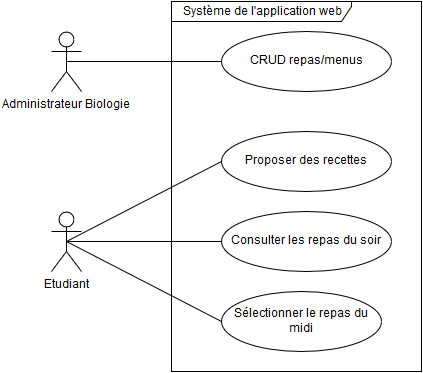
\includegraphics[width=14cm]{images/UseCase.png}}



\subsection{Scénarios}

\subsubsection{Proposer des recettes} 

Scénario nominal :
L'utilisateur sélectionne "proposer une recette" dans le menu de l'application. Ensuite il sélectionne les différents ingrédients avec leur quantité et il indique les étapes à suivre pour réaliser la recette. Pour finir il enregistre la recette

Autres scénarios :
\begin{itemize}
\item Si l'utilisateur ne trouve pas un ingrédient, il a la possibilité d'en ajouter.
\item Si l'utilisateur n'a pas pu enregistrer la recette, les éléments saisis sont enregistrés pour la prochaine fois
\end{itemize}


\subsubsection{Consulter les repas du soir} 

Scénario nominal :
L'utilisateur sélectionne "Les repas du soir" dans le menu de l'application. Par la suite il découvre les différentes recettes proposées en fonction du repas de midi.

Autres scénarios :
\begin{itemize}
\item Si le repas du midi n'a pas été renseigné, un message lui indique de renseigner le repas pris. Une liste de recette est néanmoins disponible.
\end{itemize}

\subsubsection{Ajouter/ Supprimer une recette} 

Scénario nominal :
L'utilisateur demande l'accès à la partie administration. Après s'être identifié, il sélectionne "Confirmer une recette" dans le menu de l'application. Ensuite l'administrateur peut sélectionner une recette saisie par un utilisateur pour la confirmer ou la supprimer.

Autres scénarios :
\begin{itemize}
\item Si l'identification de l'administrateur n'est pas correcte, le système renvoie un message d'erreur.
\item Si l'administrateur ne confirme pas l'ajout ou la suppression de la recette aucune action est effectué à celle-ci.
\end{itemize}


\subsubsection{Sélectionner le repas du midi} 


Scénario nominal :
Lorsque l'utilisateur lance l'application, l'utilisateur choisir à l'aide d'une liste des plats du Crous son entrée, son plat puis son dessert. Une fois qu'il aura fait son choix, son menu se verra attribué une note nutritionnel ainsi que son prix. L'utilisateur aura la possibilité de modifier son menu. Une fois que l'utilisateur a confirmé son choix, une liste des repas du soir lui est proposée.


Autres scénarios :
\begin{itemize}
\item Les éléments qui ne sont pas pris en compte par rapport aux préférences de l'utilisateur reste disponible mais ne sont pas mis en avant.
\item Deux propositions doivent au minimum être proposées.
\end{itemize}

\section{Diagramme de classe}

\includegraphics[width=15cm]{images/class_diagramme.png}

\section{Mock-up}

\subsection{Ecran d'accueil}

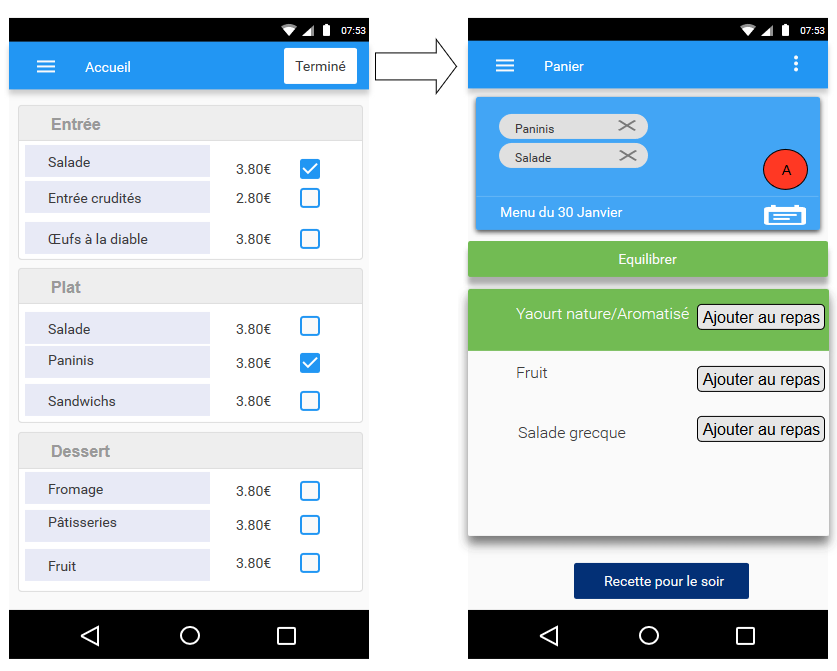
\includegraphics[width=14cm]{images/mockup_v2.png}



